\documentclass[11pt,letterpaper]{article}

% ============================================================================
% PACKAGES
% ============================================================================
\usepackage[utf8]{inputenc}
\usepackage[T1]{fontenc}
\usepackage{mathptmx}
\usepackage{amsmath,amssymb,amsthm}
\usepackage{graphicx}
\usepackage{booktabs}
\usepackage{natbib}
\usepackage[margin=1in]{geometry}
\usepackage{hyperref}
\usepackage{xcolor}
\usepackage{float}
\usepackage{algorithm}
\usepackage{algorithmic}
\usepackage{setspace}
\usepackage{longtable}

\hypersetup{
    colorlinks=true,
    linkcolor=blue!60!black,
    citecolor=blue!60!black,
    urlcolor=blue!60!black
}

\onehalfspacing

% Theorem environments with S prefix
\newtheorem{theoremS}{Theorem S}
\newtheorem{propositionS}[theoremS]{Proposition S}
\newtheorem{lemmaS}[theoremS]{Lemma S}
\newtheorem{corollaryS}[theoremS]{Corollary S}
\theoremstyle{definition}
\newtheorem{definitionS}{Definition S}
\newtheorem{assumptionS}{Assumption S}

% Custom commands
\newcommand{\E}{\mathbb{E}}
\newcommand{\R}{\mathbb{R}}

% ============================================================================
% TITLE
% ============================================================================

\title{\Large\textbf{Supplementary Information}\\[0.5em]
\large Equity implications of federal--local cost-sharing in flood buyouts}

\author{}
\date{}

% ============================================================================
% DOCUMENT
% ============================================================================

\begin{document}

\maketitle

\tableofcontents
\clearpage

% ============================================================================
\section{Model Details}
% ============================================================================

\subsection{Complete Model Specification}

We present the complete mathematical specification of the three-level stochastic Stackelberg game.

\begin{definitionS}[Game Structure]
The game $\Gamma$ consists of the following elements:

\textbf{Players.} The federal government $F$ acts as Stackelberg leader. Local governments $j \in \mathcal{J} = \{1, \ldots, J\}$ act as intermediate followers. Homeowners $h \in \mathcal{H} = \bigcup_{j} \mathcal{H}_j$ act as ultimate followers, where $\mathcal{H}_j$ denotes households in jurisdiction $j$.

\textbf{Actions.} The federal government chooses cost-sharing ratio $\alpha \in [\underline{\alpha}, \bar{\alpha}]$ and maximum subsidy cap $\bar{S} \geq 0$. Each local government $j$ chooses participation indicator $I_j \in \{0, 1\}$ and subsidy level $S_j \in [0, \bar{S}]$. Each household $h$ chooses relocation year $k_h \in \{0, 1, \ldots, T\} \cup \{\infty\}$, where $k_h = \infty$ indicates never relocating.

\textbf{Information.} All players observe the federal policy $(\alpha, \bar{S})$. Households observe their local government's participation decision and subsidy offer. Climate scenarios $\omega \in \Omega$ are realised after all decisions, with probabilities $\pi(\omega)$ common knowledge.
\end{definitionS}

\begin{assumptionS}[Climate Scenarios]\label{ass:climate}
The set of climate scenarios $\Omega = \{\omega_1, \omega_2, \omega_3\}$ corresponds to Representative Concentration Pathways:
\begin{align}
\omega_1 &: \text{RCP 2.6, sea-level rise } \delta_T^{(1)} = 0.4\text{m by 2100}, \quad \pi(\omega_1) = 0.2 \\
\omega_2 &: \text{RCP 4.5, sea-level rise } \delta_T^{(2)} = 0.6\text{m by 2100}, \quad \pi(\omega_2) = 0.5 \\
\omega_3 &: \text{RCP 8.5, sea-level rise } \delta_T^{(3)} = 1.0\text{m by 2100}, \quad \pi(\omega_3) = 0.3
\end{align}
Sea-level rise follows a quadratic trajectory $\delta_t^{(\omega)} = a^{(\omega)} t^2 + b^{(\omega)} t$ calibrated to match RCP projections.
\end{assumptionS}

\begin{assumptionS}[Homeowner Heterogeneity]\label{ass:heterogeneity}
Homeowners are characterised by type $\theta_h = (V_h, r_h, \ell_h)$ where:
\begin{align}
V_h &\in [V^{\min}, V^{\max}] : \text{total house value} \\
r_h &\in \{r^{\text{low}}, r^{\text{high}}\} : \text{discount rate, with } r^{\text{low}} < r^{\text{high}} \\
\ell_h &: \text{location determining flood exposure}
\end{align}
Low-income households have discount rate $r^{\text{high}}$ due to credit constraints; high-income households have discount rate $r^{\text{low}}$.
\end{assumptionS}

\subsection{Homeowner's Problem}

Given local government $j$'s subsidy offer $S_j$, household $h \in \mathcal{H}_j$ solves:
\begin{equation}\label{eq:homeowner_full}
\min_{k_h \geq 0} \left\{ \frac{M_h - S_j}{(1+r_h)^{k_h}} + \sum_{t=0}^{k_h-1} \frac{\E_\omega[\E[D_{h,t}^{(\omega)}]]}{(1+r_h)^t} \right\}
\end{equation}
where $M_h = V_h + C_h^{\text{mov}} + C_h^{\text{psych}}$ is total relocation cost (house value plus moving costs plus psychic costs of dislocation), and $D_{h,t}^{(\omega)}$ is flood damage in year $t$ under scenario $\omega$.

The expected annual flood damage is:
\begin{equation}
\E[D_{h,t}^{(\omega)}] = \int_0^{\infty} D_h(z) \cdot f_{h,t}^{(\omega)}(z) \, dz
\end{equation}
where $D_h(z) = V_h^{\text{str}} \cdot d(z)$ is the depth-damage function (structure value times proportional damage) and $f_{h,t}^{(\omega)}(z)$ is the probability density of flood depth.

\subsection{Local Government's Problem}

Local government $j$ solves:
\begin{equation}\label{eq:local_full}
\min_{I_j \in \{0,1\}, S_j \leq \bar{S}} \quad I_j \cdot \Phi_j(S_j) + (1 - I_j) \cdot \Phi_j^0
\end{equation}
where the participation cost is:
\begin{equation}
\Phi_j(S_j) = (1-\alpha) S_j N_j^{\text{rel}}(S_j) + C_j^{\text{admin}} + \E_\omega[C_{j}^{\text{loc},(\omega)}(S_j)] + \lambda_j \Delta TB_j(S_j)
\end{equation}
and the non-participation cost is:
\begin{equation}
\Phi_j^0 = \E_\omega[C_{j}^{\text{loc},(\omega)}(0)]
\end{equation}

Here $N_j^{\text{rel}}(S_j) = |\{h \in \mathcal{H}_j : k_h^*(S_j) < \infty\}|$ is the number of households that relocate, $C_j^{\text{admin}}$ is administrative cost, $C_{j}^{\text{loc},(\omega)}(S_j)$ is local disaster-related cost, and $\Delta TB_j(S_j) = \tau \sum_{h: k_h^* < \infty} V_h / r_L$ is the present value of lost property tax revenue.

\subsection{Federal Government's Problem}

The federal government solves:
\begin{equation}\label{eq:federal_full}
\begin{aligned}
\min_{\alpha, \bar{S}} \quad & \E_\omega\left[\sum_{j \in \mathcal{J}} \left(\alpha S_j^*(\alpha, \bar{S}) N_j^{\text{rel},*} + C_j^{\text{Fed},(\omega)}\right)\right] \\
\text{s.t.} \quad & \sum_{j} \alpha S_j^* N_j^{\text{rel},*} \leq B^{\text{Fed}} \\
& \frac{N_{\text{low}}^{\text{rel},*} / N_{\text{low}}^{\text{total}}}{N_{\text{high}}^{\text{rel},*} / N_{\text{high}}^{\text{total}}} \geq \theta \\
& \alpha \in [\underline{\alpha}, \bar{\alpha}], \quad \bar{S} \geq 0
\end{aligned}
\end{equation}
where $B^{\text{Fed}}$ is the federal budget, $\theta$ is the equity threshold, and stars denote equilibrium values.

% ============================================================================
\section{Equilibrium Analysis}
% ============================================================================

\subsection{Homeowner Equilibrium}

\begin{theoremS}[Homeowner Best Response]\label{thm:homeowner}
Under Assumptions S\ref{ass:climate}--S\ref{ass:heterogeneity}, for any subsidy $S_j \geq 0$:

(a) A unique optimal relocation year $k_h^*(S_j)$ exists for each household $h$.

(b) $k_h^*(S_j)$ is non-increasing in $S_j$ and non-decreasing in $r_h$.

(c) The subsidy required to induce relocation in year $k$ for household $h$ is:
\begin{equation}
S_h^{\text{induce}}(k) = M_h - \sum_{t=k}^{\infty} \frac{\E_\omega[\E[D_{h,t}^{(\omega)}]]}{(1+r_h)^{t-k}}
\end{equation}
which is increasing in $r_h$.
\end{theoremS}

\begin{proof}
\textbf{Part (a).} The objective function in \eqref{eq:homeowner_full} can be written as $J_h(k) = g(k) + f(k)$ where $g(k) = (M_h - S_j)/(1+r_h)^k$ is strictly decreasing in $k$ and $f(k) = \sum_{t=0}^{k-1} \E_\omega[\E[D_{h,t}^{(\omega)}]]/(1+r_h)^t$ is strictly increasing in $k$ (under Assumption S\ref{ass:climate}, expected damages are non-decreasing over time). As $k \to 0$, $J_h(0) = M_h - S_j$. As $k \to \infty$, $J_h(k) \to \sum_{t=0}^{\infty} \E_\omega[\E[D_{h,t}^{(\omega)}]]/(1+r_h)^t$. Since one component is strictly decreasing and the other strictly increasing, there exists a unique minimiser.

\textbf{Part (b).} For the subsidy effect: increasing $S_j$ shifts $g(k)$ down uniformly, making the crossing point occur at weakly smaller $k$. For the discount rate effect: consider households $h_1, h_2$ with $r_{h_1} < r_{h_2}$ and identical other characteristics. The cumulative damage term for $h_2$ is smaller at each $k$:
\begin{equation}
\sum_{t=0}^{k-1} \frac{\E[D_t]}{(1+r_{h_2})^t} < \sum_{t=0}^{k-1} \frac{\E[D_t]}{(1+r_{h_1})^t}
\end{equation}
This means higher discount rate households perceive lower cumulative damage costs, shifting optimal relocation later.

\textbf{Part (c).} At the indifference point for relocation in year $k$:
\begin{equation}
M_h - S_j = \sum_{t=k}^{\infty} \frac{\E_\omega[\E[D_{h,t}^{(\omega)}]]}{(1+r_h)^{t-k}}
\end{equation}
Solving for $S_j$ and noting that the RHS is decreasing in $r_h$ (higher discount rates reduce the sum), we obtain $S_h^{\text{induce}}(k)$ increasing in $r_h$.
\end{proof}

\begin{corollaryS}[Discount Rate Gap]\label{cor:gap}
The additional subsidy required to induce a low-income household (with $r^{\text{high}}$) to relocate in the same year as an otherwise identical high-income household (with $r^{\text{low}}$) is:
\begin{equation}
\Delta S_h = \sum_{t=k}^{\infty} \E_\omega[\E[D_{h,t}^{(\omega)}]] \left[\frac{1}{(1+r^{\text{low}})^{t-k}} - \frac{1}{(1+r^{\text{high}})^{t-k}}\right] > 0
\end{equation}
\end{corollaryS}

\subsection{Local Government Equilibrium}

\begin{assumptionS}[Regularity Conditions]\label{ass:regularity}
The aggregate relocation function $N_j^{\text{rel}}(S_j)$ is continuous and weakly increasing. Local disaster costs $C_j^{\text{loc}}(S_j)$ are convex and decreasing in $S_j$. The local government's objective function $\Phi_j(S_j)$ is strictly convex in $S_j$.
\end{assumptionS}

\begin{theoremS}[Local Government Best Response]\label{thm:local}
Under Assumptions S\ref{ass:climate}--S\ref{ass:regularity}, for any federal policy $(\alpha, \bar{S})$:

(a) There exists a unique best response $(I_j^*, S_j^*)$ for each local government $j$.

(b) The participation threshold is:
\begin{equation}
\alpha_j^{\text{crit}} = 1 - \frac{\E_\omega[C_j^{\text{loc}}(0) - C_j^{\text{loc}}(\bar{S})] - \lambda_j \Delta TB_j(\bar{S}) - C_j^{\text{admin}}}{\bar{S} \cdot N_j^{\text{rel}}(\bar{S})}
\end{equation}

(c) The equilibrium subsidy $S_j^*$ is increasing in $\alpha$: $\partial S_j^* / \partial \alpha > 0$.
\end{theoremS}

\begin{proof}
\textbf{Part (a).} Under Assumption S\ref{ass:regularity}, $\Phi_j(S_j)$ is strictly convex, ensuring uniqueness of the interior solution. The participation decision follows from comparing $\Phi_j(S_j^*) + C_j^{\text{admin}}$ with $\Phi_j^0$.

\textbf{Part (b).} At the threshold, the local government is indifferent:
\begin{equation}
(1-\alpha_j^{\text{crit}})\bar{S} N_j^{\text{rel}}(\bar{S}) + C_j^{\text{admin}} + \E_\omega[C_j^{\text{loc}}(\bar{S})] + \lambda_j \Delta TB_j(\bar{S}) = \E_\omega[C_j^{\text{loc}}(0)]
\end{equation}
Rearranging yields the expression for $\alpha_j^{\text{crit}}$.

\textbf{Part (c).} The first-order condition for interior $S_j^*$ is:
\begin{equation}
(1-\alpha)[N_j^{\text{rel}}(S_j) + S_j N_j^{\text{rel}\prime}(S_j)] + \frac{\partial \E_\omega[C_j^{\text{loc}}]}{\partial S_j} + \lambda_j \frac{\partial \Delta TB_j}{\partial S_j} = 0
\end{equation}
Define $H(S_j, \alpha)$ as the LHS. By the implicit function theorem:
\begin{equation}
\frac{\partial S_j^*}{\partial \alpha} = -\frac{\partial H / \partial \alpha}{\partial H / \partial S_j} = \frac{N_j^{\text{rel}} + S_j N_j^{\text{rel}\prime}}{\partial H / \partial S_j}
\end{equation}
Under strict convexity (Assumption S\ref{ass:regularity}), $\partial H / \partial S_j > 0$. Since $N_j^{\text{rel}} + S_j N_j^{\text{rel}\prime} > 0$ for reasonable parameters, $\partial S_j^* / \partial \alpha > 0$.
\end{proof}

\subsection{Federal Equilibrium}

\begin{theoremS}[Existence of Equilibrium]\label{thm:existence}
Under Assumptions S\ref{ass:climate}--S\ref{ass:regularity} and standard compactness conditions, there exists an optimal federal policy $(\alpha^*, \bar{S}^*)$ solving \eqref{eq:federal_full}.
\end{theoremS}

\begin{proof}
The federal objective function is continuous in $(\alpha, \bar{S})$ given continuity of local governments' best responses (Theorem S\ref{thm:local}) and homeowners' best responses (Theorem S\ref{thm:homeowner}). The constraint set $[\underline{\alpha}, \bar{\alpha}] \times [0, \bar{S}^{\max}]$ is compact. By the Weierstrass extreme value theorem, a minimum exists.
\end{proof}

% ============================================================================
\section{Equity Analysis}
% ============================================================================

\subsection{Equity Metrics}

\begin{definitionS}[Equity Metrics]
We employ four metrics to assess distributional outcomes:

\textbf{Relocation Ratio Gap (RRG):}
\begin{equation}
\text{RRG} = \frac{N_{\text{low}}^{\text{rel}} / N_{\text{low}}^{\text{total}}}{N_{\text{high}}^{\text{rel}} / N_{\text{high}}^{\text{total}}}
\end{equation}
Values below 1 indicate low-income households are underserved.

\textbf{Timing Gap (TG):}
\begin{equation}
\text{TG} = \bar{k}_{\text{low}}^* - \bar{k}_{\text{high}}^*
\end{equation}
where $\bar{k}^*$ denotes mean relocation year. Positive values indicate low-income households relocate later.

\textbf{Expected Damage Ratio (EDR):}
\begin{equation}
\text{EDR} = \frac{\E[\sum_{h \in \mathcal{H}^{\text{low}}} D_h]}{\E[\sum_{h \in \mathcal{H}^{\text{high}}} D_h]}
\end{equation}
Values above 1 indicate low-income households bear disproportionate damage.

\textbf{Subsidy Gini:} Gini coefficient of subsidy distribution across all relocated households.
\end{definitionS}

\subsection{Sources of Inequity}

\begin{theoremS}[Three Channels of Inequity]\label{thm:channels}
Under equilibrium, inequity in buyout outcomes ($\text{RRG} < 1$) arises from three channels:

(i) \textbf{Discount Rate Channel:} Low-income households' higher discount rates make subsidies less effective at inducing relocation.

(ii) \textbf{Tax-Base Preservation Channel:} Local governments' incentive to preserve tax base creates complex targeting dynamics.

(iii) \textbf{Participation Channel:} Communities with higher $\alpha_j^{\text{crit}}$ (often lower-income communities) may not participate.
\end{theoremS}

\begin{proof}
(i) From Corollary S\ref{cor:gap}, uniform subsidies induce later relocation for households with higher discount rates. Since low-income households have $r^{\text{high}} > r^{\text{low}}$, they relocate later or not at all.

(ii) From Theorem S\ref{thm:local}, local governments with $\lambda_j > 0$ face marginal tax-base loss $\lambda_j \tau V_h / r_L$ from buying out property with value $V_h$. This creates targeting incentives, though the relationship to income is not monotonic.

(iii) From Theorem S\ref{thm:local}(b), communities with higher administrative costs or stronger tax-base concerns have higher $\alpha_j^{\text{crit}}$. These characteristics often correlate with lower-income communities.
\end{proof}

\begin{propositionS}[Effect of Cost-Share Ratio on Equity]
Higher federal cost-share ratios improve the relocation ratio gap:
\begin{equation}
\frac{\partial \text{RRG}}{\partial \alpha} \geq 0
\end{equation}
\end{propositionS}

\begin{proof}
Higher $\alpha$ increases equilibrium subsidies (Theorem S\ref{thm:local}(c)), benefiting low-income households disproportionately. Additionally, higher $\alpha$ induces participation by communities with higher $\alpha_j^{\text{crit}}$.
\end{proof}

% ============================================================================
\section{Computational Algorithm}
% ============================================================================

\begin{algorithm}[H]
\caption{Solving the Three-Level Stochastic Stackelberg Game}
\label{alg:solve}
\begin{algorithmic}[1]
\REQUIRE Parameter values, climate scenarios $\Omega$, household data $\{\theta_h\}$
\ENSURE Optimal $(\alpha^*, \bar{S}^*)$, equilibrium outcomes

\STATE \textbf{Initialize:} $\alpha_{\text{grid}} = \{0.50, 0.55, \ldots, 1.00\}$, $\bar{S}_{\text{grid}} = \{0, 50000, \ldots, 500000\}$

\FOR{each $(\alpha, \bar{S})$ in grid}
    \FOR{each climate scenario $\omega \in \Omega$}
        \FOR{each jurisdiction $j \in \mathcal{J}$}
            \STATE Compute local government best response:
            \STATE \quad $S_j^* \leftarrow \arg\min_{S_j \leq \bar{S}} \Phi_j(S_j; \alpha, \omega)$
            \STATE \quad $I_j^* \leftarrow \mathbf{1}\{\Phi_j(S_j^*) + C_j^{\text{admin}} < \Phi_j^0\}$
            \IF{$I_j^* = 1$}
                \FOR{each household $h \in \mathcal{H}_j$}
                    \STATE Compute $k_h^*(S_j^*)$ via threshold condition
                \ENDFOR
            \ENDIF
        \ENDFOR
        \STATE Record outcomes for scenario $\omega$
    \ENDFOR
    \STATE Aggregate across scenarios weighted by $\pi(\omega)$
    \STATE Compute RRG, federal cost, and other metrics
\ENDFOR

\STATE $(\alpha^*, \bar{S}^*) \leftarrow \arg\min \text{FederalCost}(\alpha, \bar{S})$ s.t. $\text{RRG} \geq \theta$

\RETURN $(\alpha^*, \bar{S}^*)$ and equilibrium outcomes
\end{algorithmic}
\end{algorithm}

The algorithm runs in $O(|\alpha_{\text{grid}}| \times |\bar{S}_{\text{grid}}| \times |\Omega| \times J \times \max_j |\mathcal{H}_j|)$ time. For our implementation with 11 $\alpha$ values, 11 $\bar{S}$ values, 3 scenarios, 12 jurisdictions, and approximately 3,000 households per jurisdiction, runtime is approximately 3--5 minutes on a standard laptop.

% ============================================================================
\section{Parameter Calibration}
% ============================================================================

\subsection{Discount Rates}

We follow the literature on personal discount rates, particularly \citet{warner2001personal} who estimate discount rates from military downsizing programmes. Their estimates range from 0--30\%, with lower-income individuals exhibiting higher rates due to credit constraints. We set $r^{\text{low}} = 12\%$ and $r^{\text{high}} = 18\%$, within the range of empirical estimates. \citet{hausman1979individual} finds similar magnitudes in energy-efficiency contexts.

\subsection{Climate Scenarios}

Climate scenario probabilities and sea-level rise trajectories derive from IPCC SROCC (2019). We use local sea-level rise projections for each region from NOAA's Sea Level Rise Technical Report, adjusting for regional factors including land subsidence and ocean dynamics.

\subsection{Depth-Damage Functions}

We implement US Army Corps of Engineers depth-damage functions from IWR Report 92-R-1:
\begin{align}
d(z) = \begin{cases}
0.15 & z < 0.3\text{m} \\
0.15 + 0.30 \cdot (z - 0.3)/0.9 & 0.3\text{m} \leq z < 1.2\text{m} \\
0.45 + 0.25 \cdot (z - 1.2)/1.2 & 1.2\text{m} \leq z < 2.4\text{m} \\
\min(0.70 + 0.05 \cdot (z - 2.4)/1.2, 1.0) & z \geq 2.4\text{m}
\end{cases}
\end{align}

\subsection{Regional Parameters}

Table S\ref{tab:regional} presents calibrated parameters for each study region.

\begin{table}[H]
\centering
\caption{Regional parameter calibration}
\label{tab:regional}
\small
\begin{tabular}{lcccccc}
\toprule
Region & Households & Mean Value (\$K) & \% Low-Inc & \% 100yr FP & Elev. (m) \\
\midrule
Brooklyn, NY & 1,143 & 650 & 45\% & 35\% & 2.0 \\
Staten Island, NY & 2,850 & 580 & 52\% & 42\% & 1.8 \\
Queens, NY & 3,200 & 520 & 58\% & 65\% & 1.5 \\
Lower Manhattan, NY & 1,500 & 1,850 & 15\% & 45\% & 2.0 \\
Houston, TX & 8,500 & 285 & 55\% & 38\% & 9.0 \\
New Orleans, LA & 5,400 & 265 & 62\% & 75\% & 0.5 \\
Miami-Dade, FL & 6,200 & 485 & 48\% & 52\% & 1.5 \\
Charleston, SC & 2,600 & 425 & 42\% & 55\% & 2.5 \\
Norfolk, VA & 3,100 & 245 & 50\% & 48\% & 1.5 \\
\midrule
\textbf{Total} & \textbf{34,493} & & & & \\
\bottomrule
\end{tabular}
\end{table}

% ============================================================================
\section{Extended Data Figures}
% ============================================================================

\begin{figure}[H]
\centering
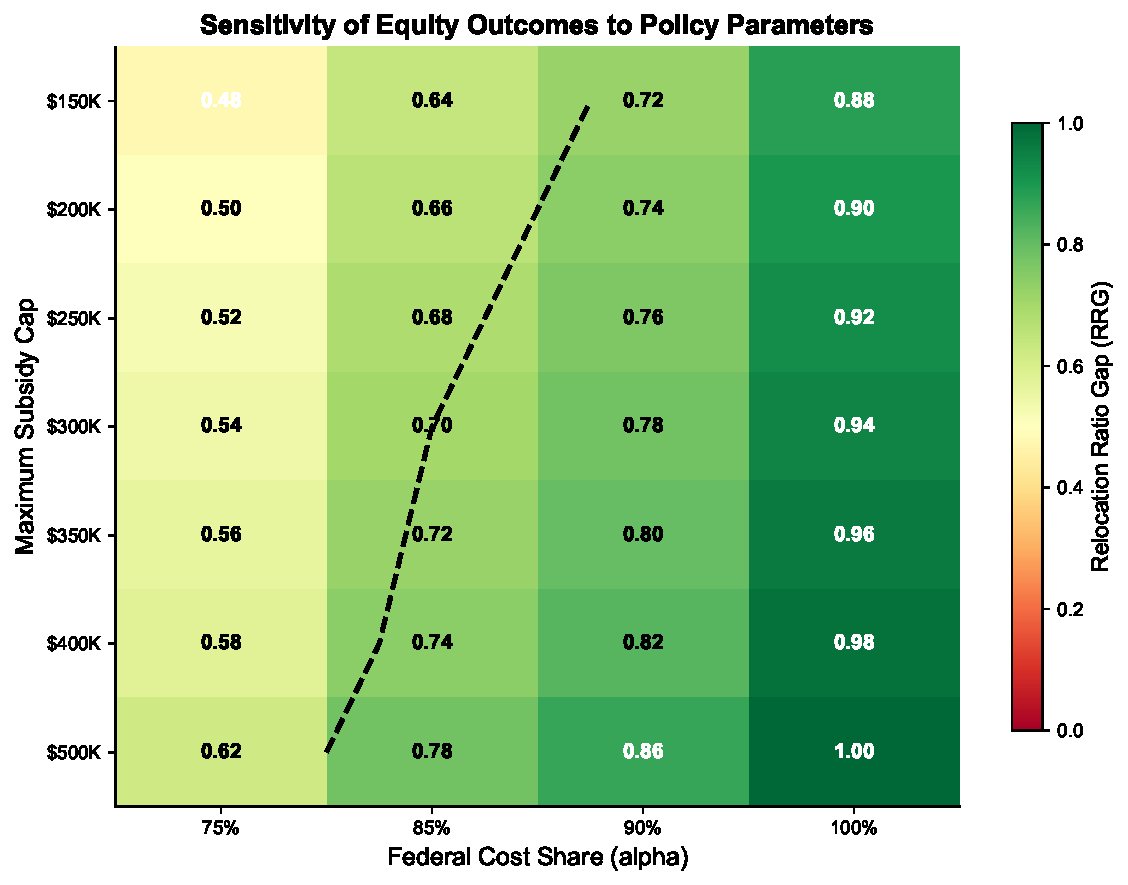
\includegraphics[width=0.75\textwidth]{../code/output/figures/fig5_sensitivity_heatmap.pdf}
\caption{\textbf{Extended Data Fig.~1: Sensitivity of equity ratio to discount rate heterogeneity and federal cost share.} Heatmap shows RRG as a function of federal cost-share ratio $\alpha$ (x-axis) and maximum subsidy cap (y-axis). Higher caps and higher federal shares both improve equity, with complementary effects visible in the interaction.}
\label{fig:ed1}
\end{figure}

% ============================================================================
\section{Robustness Checks}
% ============================================================================

\subsection{Alternative Discount Rate Specifications}

We test five discount rate scenarios to assess sensitivity:

\textbf{Base Case:} $r^{\text{low}} = 12\%$, $r^{\text{high}} = 18\%$ (baseline)

\textbf{Low Heterogeneity:} $r^{\text{low}} = 12\%$, $r^{\text{high}} = 14\%$

\textbf{High Heterogeneity:} $r^{\text{low}} = 10\%$, $r^{\text{high}} = 22\%$

\textbf{Warner \& Pleeter:} $r^{\text{low}} = 10\%$, $r^{\text{high}} = 20\%$

\textbf{Extreme Credit Constraint:} $r^{\text{low}} = 8\%$, $r^{\text{high}} = 25\%$

Results show that achieving RRG $\geq 0.70$ requires $\alpha \in [0.78, 0.92]$ depending on the discount rate specification, confirming that the qualitative conclusions are robust but quantitative policy thresholds depend on this parameter.

\subsection{Alternative Climate Scenarios}

We test sensitivity to climate scenario assumptions using four specifications: Baseline (RCP 4.5), Optimistic (RCP 2.6), Pessimistic (RCP 8.5), and High SLR (1.5m by 2100). Under pessimistic scenarios, RRG under current policy ranges from 0.24 to 0.29, a modest variation that does not qualitatively change policy conclusions.

\subsection{Alternative Tax-Base Weight}

We vary the local government tax-base preservation parameter $\lambda_j$ from 0 to 0.5. Higher values reduce local subsidy offers but do not change the qualitative finding that higher federal cost shares improve equity.

% ============================================================================
% REFERENCES
% ============================================================================

\bibliographystyle{unsrtnat}
\bibliography{references}

\end{document}
